\documentclass[12pt]{../notes}

% Command for Questions
%\question{}

% Command for Notes
% \note{}

% Code to create a minipage where you can type in class notes. 
%%\begin{minipage}[l][2cm][c]{\textwidth}
%\begin{comment}

%\end{comment}
%%\end{minipage}

\usepackage{listings}

% In order for the minted code to run, we had to create a new compilation routine called pdflatex+shellEscape.
% This includes a --shell-escape command which should ONLY be used when pygmentized is required as it compromises security. 
% We also had to add pygmentize (a python package) to the system path (BEFORE miktex) and then restart the computer. 
\usepackage{minted}
\usemintedstyle{borland}
\lstset{language=SAS, 
  breaklines=true,  
  basicstyle=\ttfamily\bfseries,
  columns=fixed,
  keepspaces=true,
  identifierstyle=\color{blue}\ttfamily,
  keywordstyle=\color{cyan}\ttfamily,
  stringstyle=\color{purple}\ttfamily,
  commentstyle=\color{green}\ttfamily,
  } 
  
% \begin{minted}{sas}
% \end{minted}


% Begin Document
%==============================================================================
\begin{document}
% Include the Title of the Handout
\ntitle{4.3: Nonparametric Regression}

% Include Numbered Sections
\section{Why nonparametric regression?}
For most of this course, we have assumed models of the form:
$$Y_i = \beta_0 + \beta_1X_{i, 1} + \beta_2X_{i, 2} + \cdots + + \beta_{p-1}X_{i, p-1} + \epsilon.$$

Such models assume the following:
\bi
\item Each explanatory variable shares a linear relationship with the response variable (perhaps aided by transformations). 
\bi
\item In other words, after transformations, the rate of increase or decrease in Y is independent of the actual values of X. 
\ei
\item The effect of each explanatory variable can be isolated from the rest (assuming no interaction terms). 
\bi
\item In other words, each explanatory variable is independent of all other explanatory variables. 
\ei
\ei

\question{What are some consequences associated with inappropriately assuming a linear model?}

\begin{minipage}[l][4cm][c]{\textwidth}
%\begin{comment}
\note{
\bi
\item If residual distributional assumptions are violated, there can be no meaningful model inference. 
\item Our accuracy will likely be poor if we assume the wrong model form. 
\ei
}
%\end{comment}
\end{minipage}

\begin{figure}[H]
\centering
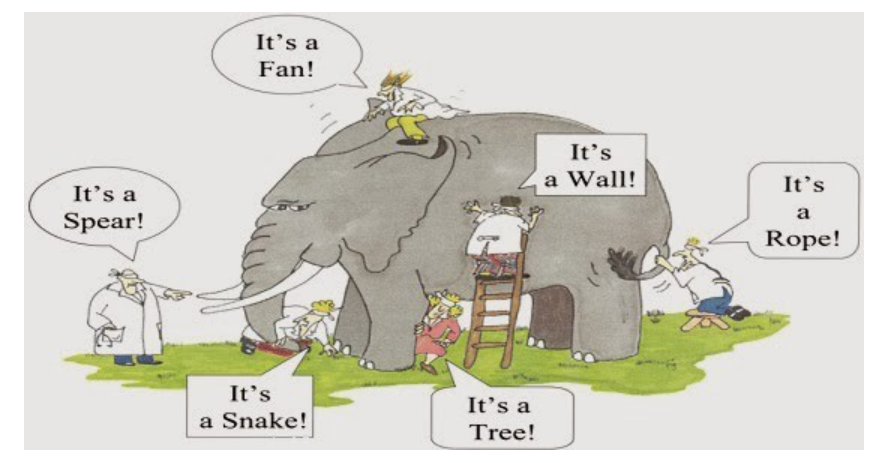
\includegraphics[width=0.7\textwidth]{../figures/module4/elephant.png}
\caption{\protect\url{https://medium.com/betterism/the-blind-men-and-the-elephant-596ec8a72a7d}}
\end{figure}

Nonparametric methods make far less (if any) assumptions about the form of the relationship between the explanatory and response variables. 

\nspace
\textbf{The cost:} Methods are often much more ``data hungry'' and harder to explain. 

\section{LOESS (\textbf{lo}cal \textbf{re}gression)}
Close relative, lowess (local weighted regression scatter plot smoothing)

\subsection{Assumptions}
\bi
\item Predictor variables are pre-selected
\item The response function is ``smooth.'' (i.e. small changes in any $X_i$, lead to relatively small changes in $Y$). 
\item Error terms are normal with constant variance. 
\ei

\subsection{Process}
In order to make a prediction $\hat{Y}$ for a particular ``X-profile'' (i.e. combination of unique values for each explanatory variable)
\begin{enumerate}
\item (optional) standardize predictor variables $X_i$
\item For each observation $i$, calculate the distance to the current X-profile $X_{h, j}$
$$d_i = \sum_{j=1}^{p-1}\left(X_{i,j} - X_{h,j}\right)^2$$
\item Let q = proportion of observations nearest to the current X-profile ($q\in (0, 1)$)
\item Let $d_q$ = distance from X-profile to the furthest observation in the neighborhood as defined by $q$
\item For each observation $i$ within that neighborhood, define weight 
$$w_i = 
\begin{cases}
\left(1-\left(\frac{d_i}{d_q}\right)^3\right)^3 & d_i < d_q \\
0 & otherwise
\end{cases}
$$
\item Using these weights, fit a weighted least squares (WLS) regression model based on polynomials of all predictors. 
\item Use the WLS model to estimate $\hat{Y}$
\bi
\item Polynomial degree:
\bi
\item 0 - moving average
\item 1 - connected lines
\item 2 - smooth curves
\item (don't typically go higher than degree 2 as this can lead to unstable fits)
\ei
\ei
\end{enumerate}

\subsection{Implementation}
LOESS requires the user to select the smoothing parameter $q$. (See Figure \ref{fig:loessCurve}.) 
\bi
\item Larger q $\rightarrow$ smoother fit
\item Smaller q $\rightarrow$ ``choppy fit''
\ei


\begin{figure}[H]
\centering
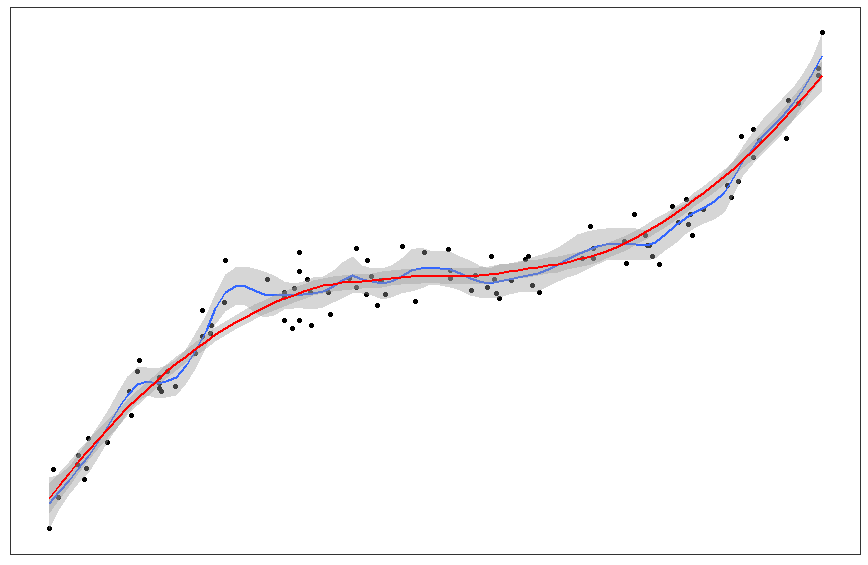
\includegraphics[width = 0.6\textwidth]{../figures/module4/loessCurve.png}
\caption{Example LOESS smoothing curves with only one X-variable and two levels of smoothness.}
\label{fig:loessCurve}
\end{figure}

\bi
\item Advantages
\bi
\item Flexible response surface - do not have to worry about whether or not the data share a linear relationship. 
\ei
\item Disadvantages:
\bi
\item Requires ``dense'' data to get good predictions. 
\bi
\item Method extremely sensitive to outliers in ``sparse'' data regions. 
\ei
\item No ``model'' to report - no inference. 
\ei
\ei

\textbf{In general, the less our model \textit{assumes}, the more data we must \textit{consume}.}

\newpage
\section{Regression Trees}
Simple, yet powerful way to handle high-ordered interactions between variables. 

\subsection{Process}
\bi
\item Separate the data into two \textbf{branches} by splitting the data in a way that minimizes the sum of squares error $\sum_i\left(Y_i - \hat{Y}_i\right)^2$ (or a similar metric). 
\bi
\item Predictions $\hat{Y}_i$ in this case is the average of the values in each \textbf{terminal node or leaf} (i.e. the group of values that fall into each branch at the end of the tree).  
\ei
\item Keep splitting the subgroups over and over until all nodes are completely \textbf{pure} ($\sum_i\left(Y_i - \hat{Y}_i\right)^2$ = 0). 
\bi
\item This may mean that each terminal node in the \textbf{fully grown} tree will be single observations. 
\ei
\item Because a model that perfectly predicts the training data is obviously overfit, we will \textbf{prune} the tree back to a set of cuts that balances accuracy with simplicity. 
\bi
\item Typically picked using a \textbf{cost complexity parameter}:
$$CC(T) = R(T) + \alpha|T|$$
\bi
\item $CC(T)$ - cost complexity
\item $R(T)$ - error rate (such as average squared error)
\item $\alpha$ - user selected cost parameter (controls size of tree). 
\item $|T|$ - number of nodes in the tree
\ei
\item Alternatively, complexity can be defined using restrictions on the tree such as:
\bi
\item Minimum number of observations in a terminal node. 
\item Minimum percentage increase in the percent variance explained in order for a split to be conducted. 
\ei
\ei
\ei

Example: predicting snow density using climate reanalysis data. 

Variables
\bi
\item maxv\_SNWD - the depth of the snowpack (mm)
\item TD - difference in the mean annual temperature between the coldest and the warmest month of the year (degrees Celsius)
\item PPTWT - total winter (Dec to Feb) precipitation. 
\ei

\begin{figure}[H]
\centering
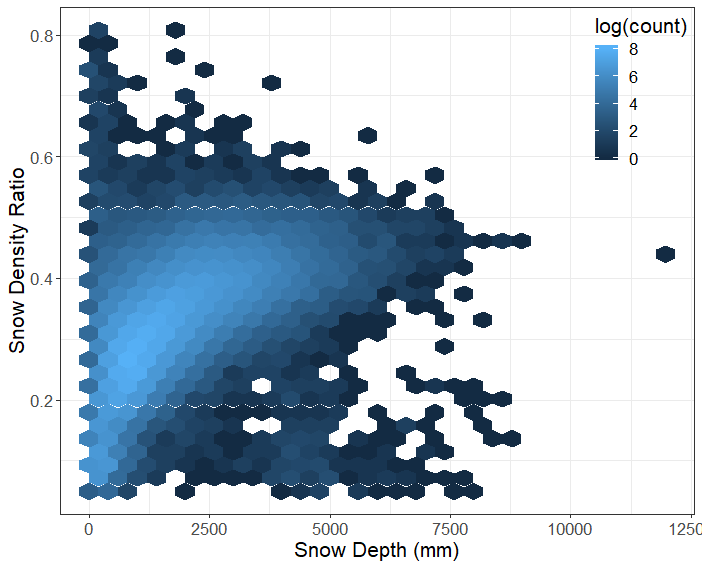
\includegraphics[width = 0.6\textwidth]{../figures/module4/snowRatio.png}
\caption{Plot of the snow density ratio in relation to its depth for locations across North America.}
\end{figure}

\begin{figure}[H]
\centering
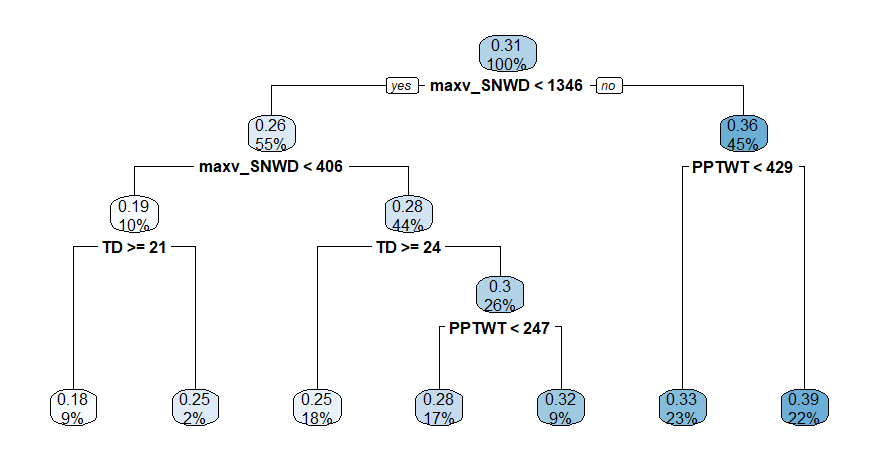
\includegraphics[width = \textwidth]{../figures/module4/sampleTree.png}
\caption{Sample tree (pruned) for predicting snow ratio using climate variables.}
\end{figure}

\subsection{Variable Importance}
There are several ways in which we can explore the importance of variables in a regression tree. 
\bi
\item \textbf{Count:} Variables that are used \textit{more often} for splitting are more important. 
\item \textbf{Error Reduction:} The greater reduction in the SSE resulting from splitting on a variable, the more important a variable. 
\ei

\subsection{Extensions of Regression Trees}
\bi
\item Boosting - fit tree in an iterative fashion, re-weighting the observations for the next split depending on the values of the residuals from the previous split. 
\bi
Essentially, a combination of ``weak'' trees that together provide a stronger prediction. 
\ei
\item Bagging - fit many trees, with each tree using a bootstrap sample of the training data. 
\bi
\item Final predictions for an observation are simply the average prediction from each tree. 
\ei
\item Methods that combine/average predictions from a group of simpler models are called ``ensemble methods.''
\ei

\question{Why might ensemble-based approaches provide better (more accurate) predictions when compared to a single regression tree?}

% Code to create a minipage where you can type in class notes. 
\begin{minipage}[l][3cm][c]{\textwidth}
%\begin{comment}
\note{Taking the \textbf{average} of a set of predictions has the effect of reducing the \textbf{variance} of the overall prediction. Reductions in variance lead to an overall increase in accuracy.}
%\end{comment}
\end{minipage}

\section{Random Forest}
A clever ensemble based method that was created by Leo Breiman and USU's own Adele Cutler. 

\nspace
An extension of bagging that, in addition to taking bootstrap samples of the original data for each tree, also only considers a random subset of the variables when deciding how to split the tree at each node. 
\bi
\item The random sub-setting of the variables helps differentiate the trees, which further reduces the variance of the predictions. 
\ei

\textbf{SAS:}

\begin{minted}{sas}
proc hpforest data=<dataset> seed=<random seed> scoreprole=oob;
input <all my explanatory variables>
target <my response variable>;
ods output <outputs you want printed to screen>
run;
\end{minted}

\subsubsection{Model Accuracy}
\bi
\item Bootstrap samples are samples with replacement from the original data, which means some observations show up more than once in each sample, and other observations do not show up at all. 
\item This means that each observation will have been ignored when creating some subset of the trees. 
\item We can determine the out of bag (OOB) error rate by making predictions using only the trees from which a particular observation was not included in the fitting. 
\ei

\subsubsection{Variable Importance}
Random Forest includes a powerful measure of variable importance:
\bi
\item For each tree, look at the OOB and random permute (scramble) the values of a single predictor variable $X_j$.
\item Pass the OOB data with the scrambled $X_j$ information down the tree - obtain the OOB error rate. 
\item Compare this error with the OOB error obtained when $X_j$ was not scrambled. 
\item The worse the error rate is with the scrambled $X_j$ information, the more important $X_j$ is to the model. 
\ei


\subsubsection{Limitations}
\bi
\item Random forests is an extremely powerful method, but is often referred to as a ``black box'' algorithm because it does not produce a model. 
\item The lack of model makes random forest more difficult to interpret. 
\item Random forests does offer \textbf{partial dependence plots}, which visualize the effect of each predictor holding all others constant, but these are not implemented in SAS. 
\item Alternatively, one can get a \textbf{generalized additive model} to try and visualize the effect of each predictor. 
$$Y_i = s_0 + s_1\left(X_{i, 1}\right) + \cdots + s_{p-1}\left(X_{i, p-1}\right) + \epsilon_i$$
\ei


\section{Helpful Resources}
(both from USU’s Dr. Richard Cutler):
\bi
\item “What Statisticians Should Know about Machine Learning'” (2017 SAS Global Forum proceedings)
\url{https://support.sas.com/resources/papers/proceedings17/0883-2017.pdf}
\item “Prediction and Interpretation for Machine Learning Regression Methods” (2018 SAS Global Forum proceedings)
\url{https://pdfs.semanticscholar.org/eade/6d9e5a9e5e3667cb2f88c665638735c8825a.pdf}
\ei





\nspace
\textbf{Remember, the less our model \textit{assumes}, the more data we must \textit{consume}.}

% End the Document
%==============================================================================
\end{document}